\section{Faulted 3-phase network (2)}
\subsection{Type of fault}
From the waveforms presented in the assignment sheet, we see that as the fault occurs, the phase A and B voltages collapse, whilst the phase C voltage remains unaffected. The phase angle of A and B becomes the same and is \SI{180}{\degree} out of phase with respect to C. In terms of the current, we see that there is a significant increase in current magnitude in phase A and B. They are also \SI{180}{\degree} out of phase with each other. The unfaulted phase remains as is. We also see that there is no significant ground current in the faulted phases.

In terms of the standard fault sequence connections, the above can be summarised as:
\begin{align}
    V_a            & = V_b       \\
    \therefore V_1 & = V_2       \\
    I_a            & = -I_b      \\
    I_c            & \ll I_a     \\
    I_0            & = 0         \\
    \therefore I_c & = I_1 + I_2
\end{align}
where subscript $a$, $b$, $c$ represents phase and subscript $1$, $2$, $0$ represents positive, negative and zero sequence. Hence, the analysis is indicative of a line-to-line fault, occurring on phases A and B.
\subsection{Breaker circuit}
\begin{figure}[H]
    \centering
    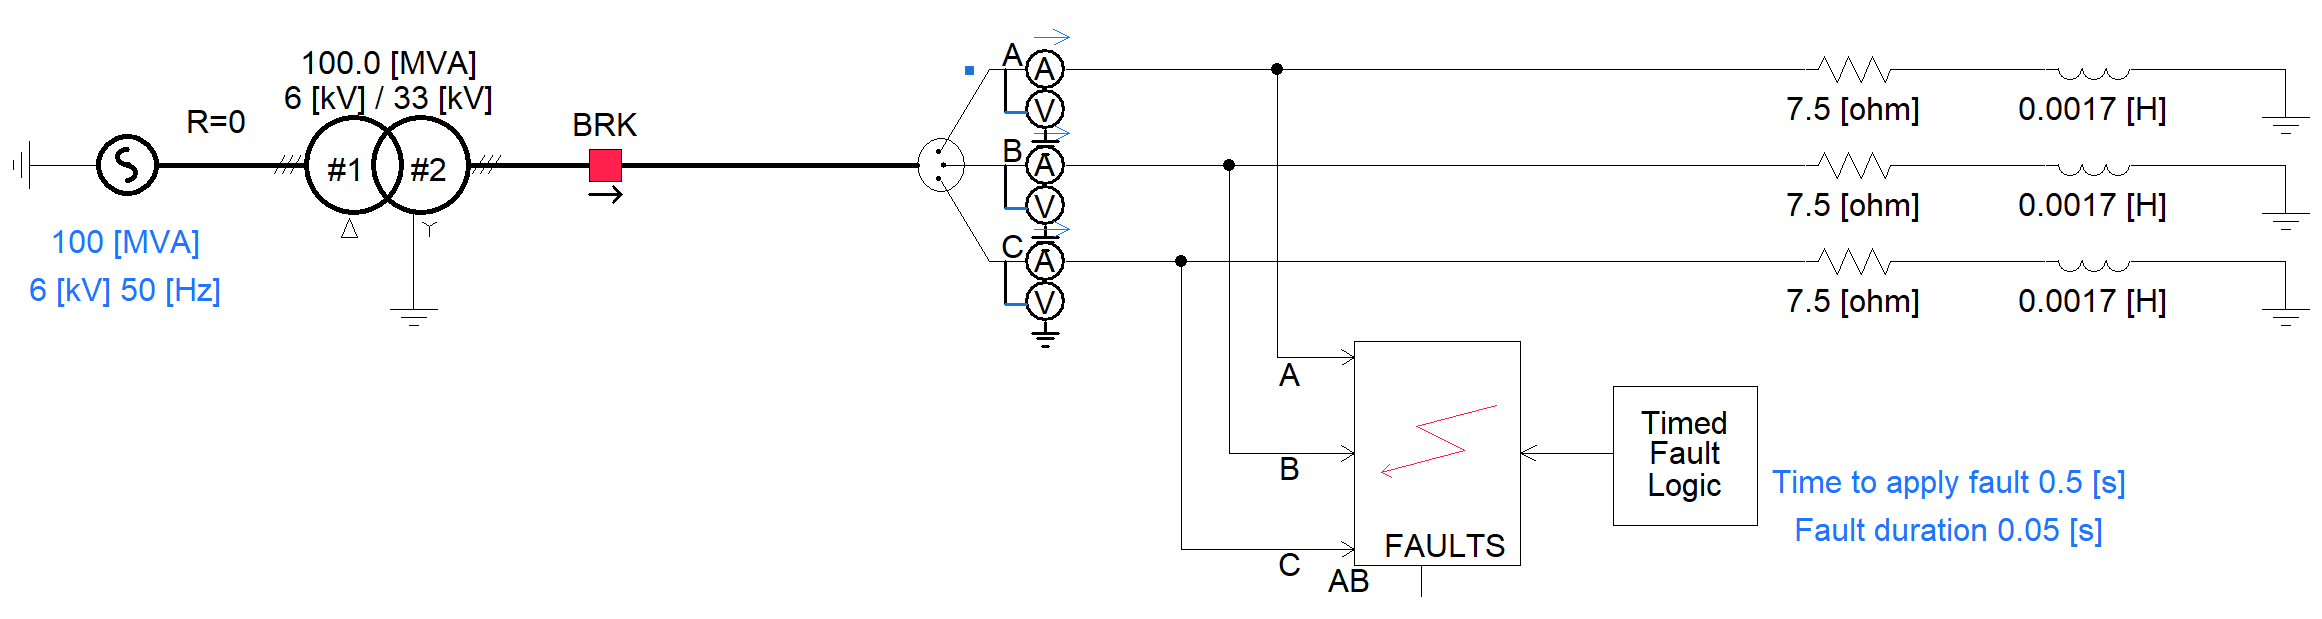
\includegraphics[width = \textwidth]{img/figure15.png}
    \caption{Circuit diagram to show distribution network with circuit breaker.}
    \label{fig:breakerNetwork}
\end{figure}
\begin{figure}[H]
    \centering
    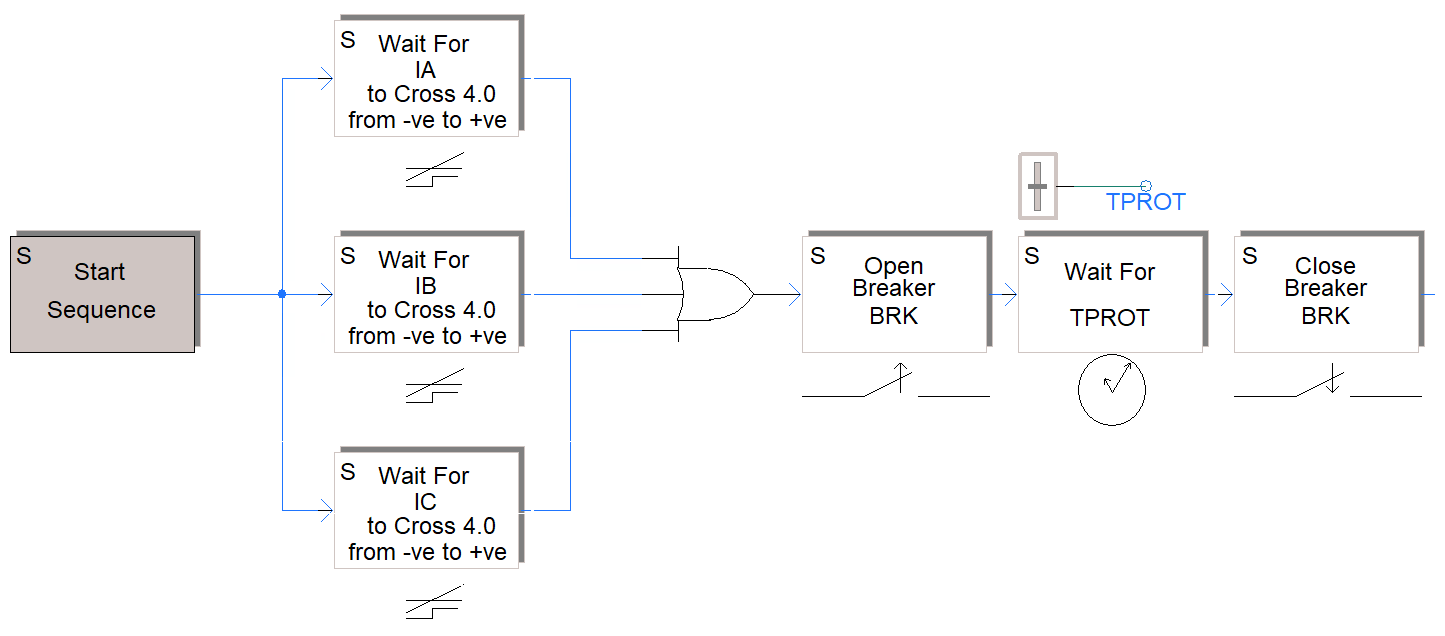
\includegraphics[width = \textwidth]{img/figure16.png}
    \caption{Sequencer diagram to show breaker activation logic.}
    \label{fig:sequencer}
\end{figure}